\documentclass[12pt,a4paper]{report}
\usepackage[latin1]{inputenc}
\usepackage{amsmath}
\usepackage{amsfonts}
\usepackage{amssymb}
\usepackage{graphicx}
\usepackage[document]{ragged2e}
\usepackage[scale=0.85,top=1cm]{geometry}
\centering
\date{ 20$^{th}$ May,2019 - 5$^{th}$ July,2019}
\title{SUMMER INTERNSHIP PROGRAM 2019}

\renewcommand{\thesection}{\arabic{section}}
\begin{document}
\renewcommand{\thesection}{\arabic{section}}
	
\begin{figure}
	\centering
	\maketitle
	{\Large \textbf{Sentiment Analysis of Amazon Reviews}}\\Final Report\\
	\includegraphics[width=0.25\linewidth]{/root/Downloads/mnitlogo}
	
	\maketitle{MALAVIYA NATIONAL INSTITUTE OF TECHNOLOGY}
	\end{figure}
\begin{figure}[h]
	\centering
	\includegraphics[width=0.25\linewidth]{/root/Downloads/ramanlogo}\\
	\maketitle{ROBOTICS AND MACHINE ANALYTICS RAMAN LAB }
\end{figure}
\begin{table}[h!]
	\begin{center}
		\maketitle
			{\large Submitted by:}\\ 
		
		\begin{tabular}{l l l l l } 

			\textbf{\Large Ujjawal Gupta} &&  &  &\textbf{\Large Shreya Jakhar}\\

			
			National Institute of &  &   &&MODY University,\\

			Technology, Hamirpur            &  &  &   &Laxmangarh             \\

			gujjawal29@gmail.com &  &&   &shreyajakhar22@gmail.com
		\end{tabular}

	\end{center}
\end{table}
\maketitle{\large Under the supervision of\\\textbf{ Prof.(Dr.) Rajesh Kumar}\\ Department of Electrical Engineering\\ Malaviya National Institute of Technology\\ Jaipur, Rajasthan, India}
%\newpage
\tableofcontents

\newpage

\section{Introduction}
\justifying
Sentiment analysis of product reviews, an application problem, has recently become very popular in text mining and computational linguistics research. Here, we want to study the correlation between the Amazon product reviews and the rating of the products given by the customers. We use both traditional machine learning algorithms including Multinomial Naive Bayes, Bernoulli Naive Bayes, Random Forest, Logistic Regression and Bagging. By comparing these results, we could get a better understanding of the these algorithms. They could also act as a supplement to other fraud scoring detection methods.


\section{Problem Development}
\justifying
Recent years have seen an increasing amount of research efforts expanded in understanding sentiment in textual resources.One of the subtopics of this research is called sentiment analysis or opinion mining, which is, given a bunch of text, we can computationally study peoples opinions, appraisals, attitudes, and emotions toward entities, individuals, issues, events, topics and their attributes.  Applications of this technique are diverse.
The  objective  of  this  paper  is  to  classify  the  positive and negative reviews of the customers over different products and build a supervised learning model to polarize large amounts of reviews.  Our dataset consists of customer's reviews and ratings.  We extracted the features of our dataset and  built  several  supervised  model  based  on  that.These models include algorithms such as Multinomial Naive Bayes, Bernoulli Naive Bayes, Random Forest, Logistic Regression and Bagging. We compared the accuracy of these models and got a better understanding of the polarized attitudes towards the products.
\section{Methodology}
\subsection{Multinomial Naive Bayes}
With a multinomial event model, samples (feature vectors) represent the frequencies with which certain events have been generated by a multinomial p\textsubscript{1}, \dots ,p\textsubscript{n} where p\textsubscript{i} is the probability that event i occurs (or K such multinomials in the multiclass case).  A feature vector x = x\textsubscript{1}, \dots ,x\textsubscript{n} is then a histogram, with x\textsubscript{i} counting the number of times event i was observed in a particular instance.  This is the event model typically used for document classification, with events representing the occurrence of a word in a single document (see bag of words assumption). The likelihood of observing a histogram x is given by:
\begin{equation}
p(\mathbf{x} \mid C_k) = \frac{(\sum_i x_i)!}{\prod_i x_i !} \prod_i {p_{ki}}^{x_i}
\end{equation}

\subsection{Bernoulli Naive Bayes}
\justifying
In the multivariate Bernoulli event model, features are independent booleans (binary variables) describing inputs. Like the multinomial model, this model is popular for document classification tasks, where binary term occurrence features are used rather than term frequencies. If x\textsubscript{i} is a boolean expressing the occurrence or absence of the i\textsuperscript{th} term from the vocabulary, then the likelihood of a document given a class C\textsubscript{k} is given by:
\begin{equation}
p(\mathbf{x} \mid C_k) = \prod_{i=1}^n p_{ki}^{x_i} (1 - p_{ki})^{(1-x_i)}
\end{equation}
Where p\textsubscript{ki} is the probability of class C\textsubscript{k} generating the term x\textsubscript{i}.This event model is especially popular for classifying short texts. It has the benefit of explicitly modelling the absence of terms.\textsubscript{i}

\subsection{Random Forest}
\justifying
Random forests or random decision forests are an ensemble learning method for classification, regression and other tasks that operates by constructing a multitude of decision trees at training time and outputting the class that is the mode of the classes (classification) or mean prediction (regression) of the individual trees.Random decision forests correct for decision trees habit of overfitting to their training set.\cite{ref3}

\begin{figure}[h]
	\centering
	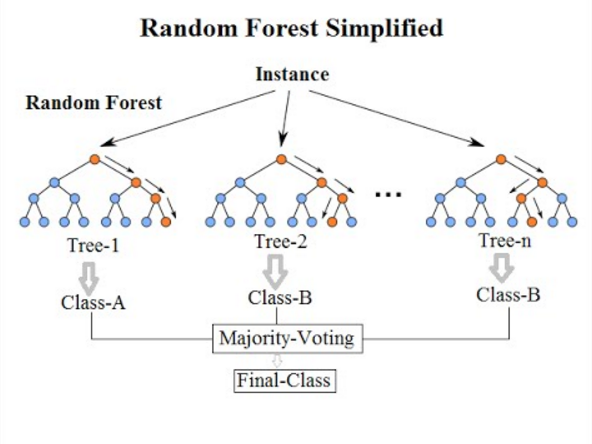
\includegraphics[width=0.75\linewidth]{/root/Downloads/random_forest}\\
	\caption{Random Forest\cite{ref4}}
\end{figure}


\subsection{Logistic Regression}
\justifying
Logistic regression is named for the function used at the core of the method, the logistic function.
The logistic function, also called the sigmoid function was developed by statisticians to describe properties of population growth in ecology, rising quickly and maxing out at the carrying capacity of the environment. It's an S-shaped curve that can take any real-valued number and map it into a value between 0 and 1, but never exactly at those limits.
Logistic regression uses an equation as the representation, very much like linear regression.
Input values (x) are combined linearly using weights or coefficient values (referred to as the Greek capital letter Beta) to predict an output value (y). A key difference from linear regression is that the output value being modeled is a binary values (0 or 1) rather than a numeric value.\cite{ref1}

\subsection{Bagging}
\justifying
Bootstrap aggregating, also called bagging, is a machine learning ensemble meta-algorithm designed to improve the stability and accuracy of machine learning algorithms used in statistical classification and regression. It also reduces variance and helps to avoid overfitting. Although it is usually applied to decision tree methods, it can be used with any type of method.Bagging is a special case of the model averaging approach. 
Given a standard training set D of size n, bagging generates m new training sets D\textsubscript{i}, each of size n', by sampling from D uniformly and with replacement. By sampling with replacement, some observations may be repeated in each D\textsubscript{i}.If n'=n, then for large n the set D\textsubscript{i} is expected to have the fraction (1 - 1/e) ($\approx$63.2\%) of the unique examples of D, the rest being duplicates.This kind of sample is known as a bootstrap sample. Then, m models are fitted using the above m bootstrap samples and combined by averaging the output (for regression) or voting (for classification).\cite{ref2}

\begin{figure}[h]
	\centering
	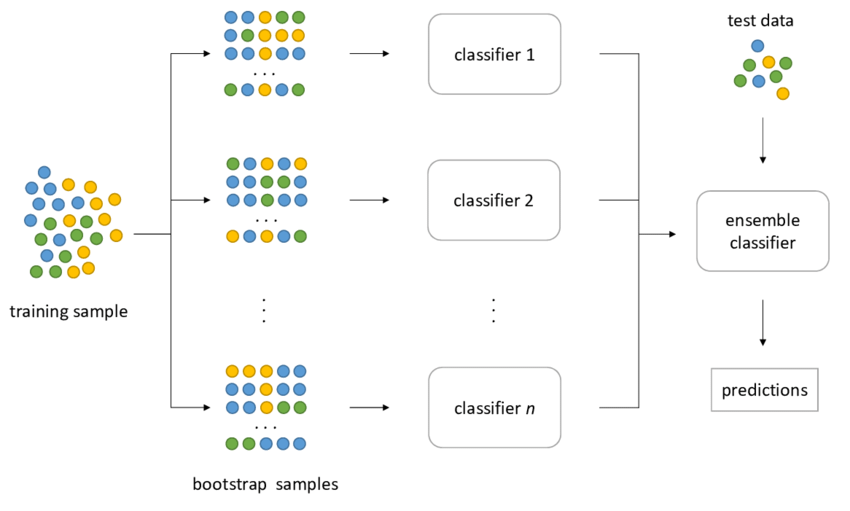
\includegraphics[width=0.75\linewidth]{/root/Downloads/bagging}\\
	\caption{Bagging\cite{ref5}}
\end{figure}


\section{Simulations and Results}
\justifying

The entire dataset of 2,96,337 reviews was divided into a training  set  of  size  217812   (80\%) and a test set of size 54454 (20\%).With 779569-d input features representing review text, we implemented Multinomial Naive Bayes, Bernoulli Naive Bayes, Random Forest, Logistic Regression and Bagging. Among all these classifiers Logistic Regression seems to perform best with 95.66\% accuracy.


\begin{table}[h!]
	\begin{center}
		\caption{Accuracy Table}
		\label{tab:table1}
		\begin{tabular}{|| c c c ||} 
		\hline
		\multicolumn{3}{|c|}{Accuracy Score} \\
		\hline
		Models & Training Acc.  & Test Acc. \\ [0.5ex] 
		\hline\hline
		Multinomial NB & 93.66\% & 93.47\% \\ 
		\hline
		Bernoulli NB & 93.18\% & 92.99\%  \\
		\hline
		Random Forest & 92.9\% & 92.9\% \\
		\hline
		Logistic Regression & 99.52\% & 95.8\% \\
		\hline
		Bagging & 95.6\% & 95.63\% \\ [1ex] 
		\hline
		\end{tabular}

	\end{center}
\end{table}

On the basis of results obtained we used Logistic Regression as our final model.We used Logistic Regression in our web interface because of its high accuracy.

\newpage

\subsection{Our Web Interface}
\justifying
In our project we felt the need of one interface to make our project more productive and efficient.So we built one interface using Python CGI and HTML.In this interface we can enter the review in the form of statements be it short or long.This interface is used by the person who is managing the site.So he can check whether the entered reviews are positive or negative.When the review is entered on the interface it will recognize the positive and negative words used in the statement and will generate the result based upon that.The result that is obtained will show the probability of positivity and negativity of that review.
	
\begin{figure}[h]
	\centering
	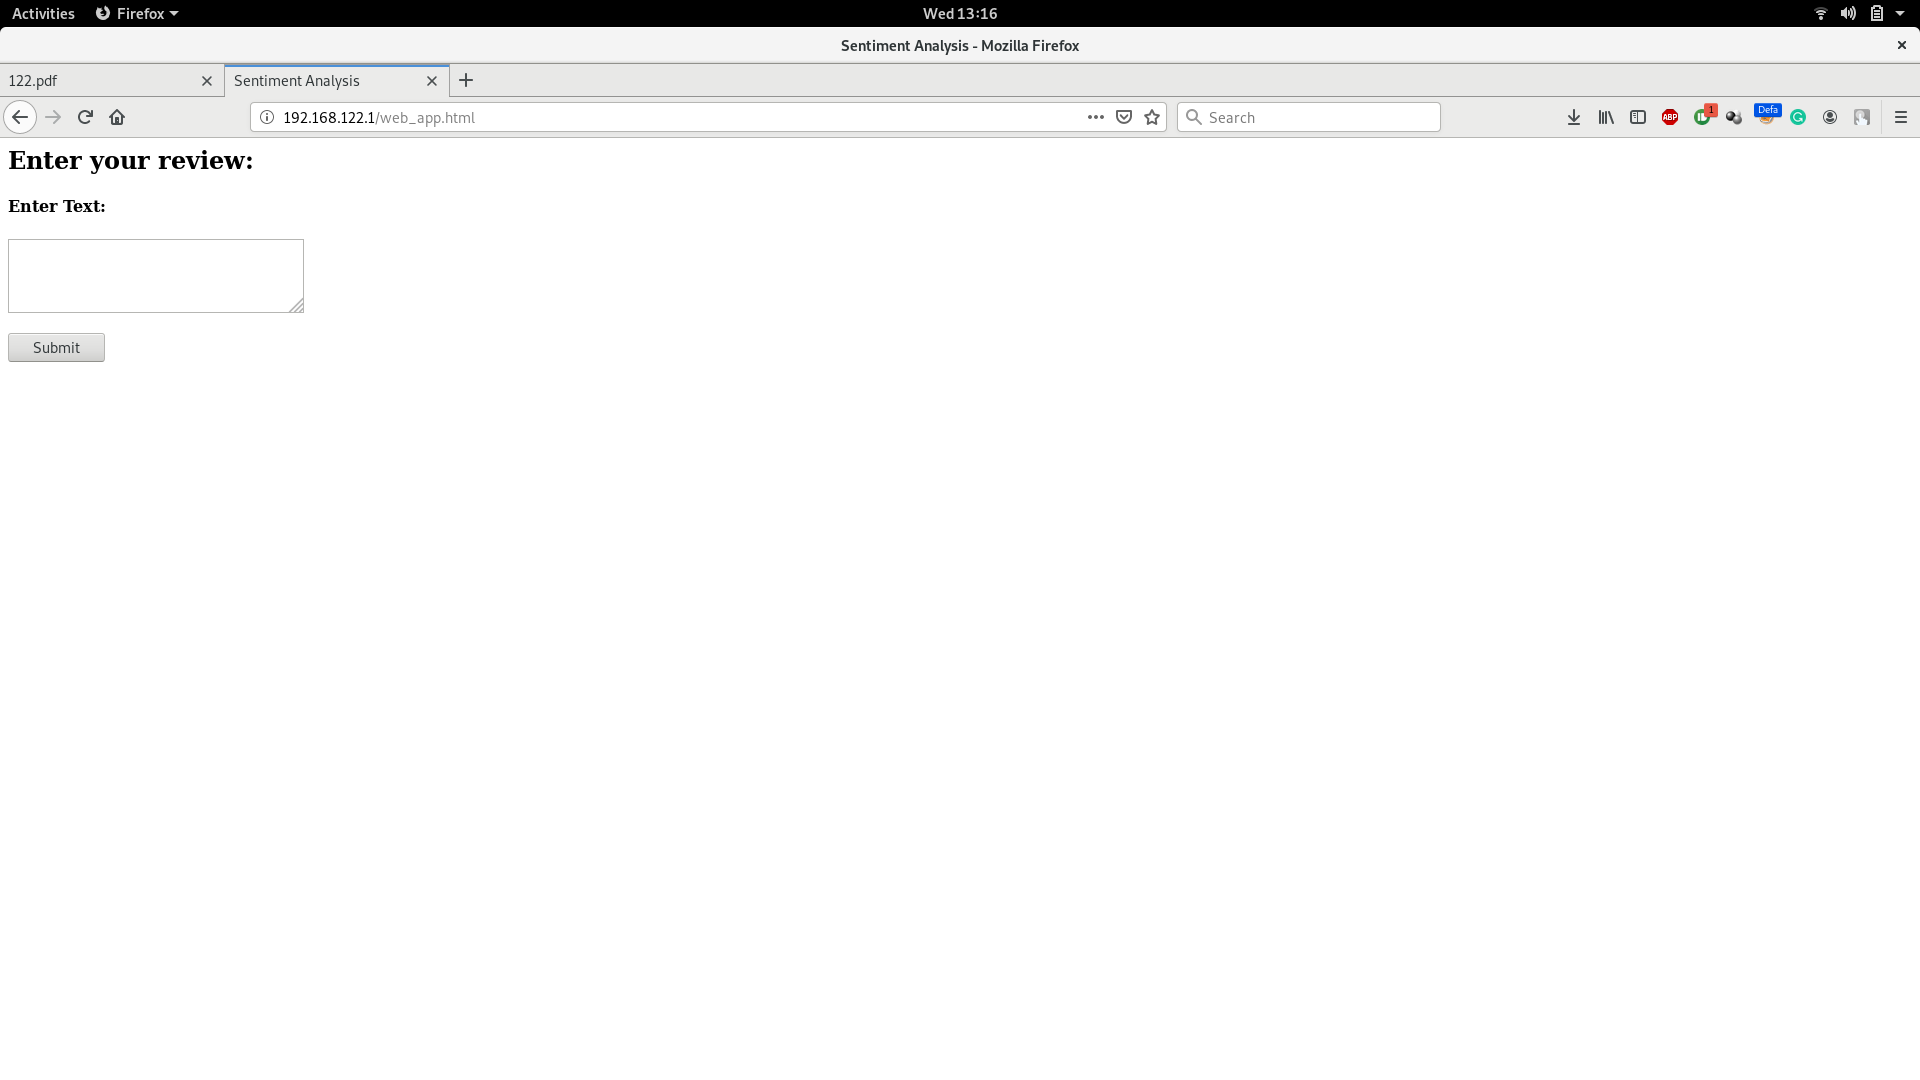
\includegraphics[height = 5cm , width=0.75\linewidth]{/root/Downloads/7}\\
	\caption{Interface}
\end{figure}


\begin{figure}[h]
	\centering
	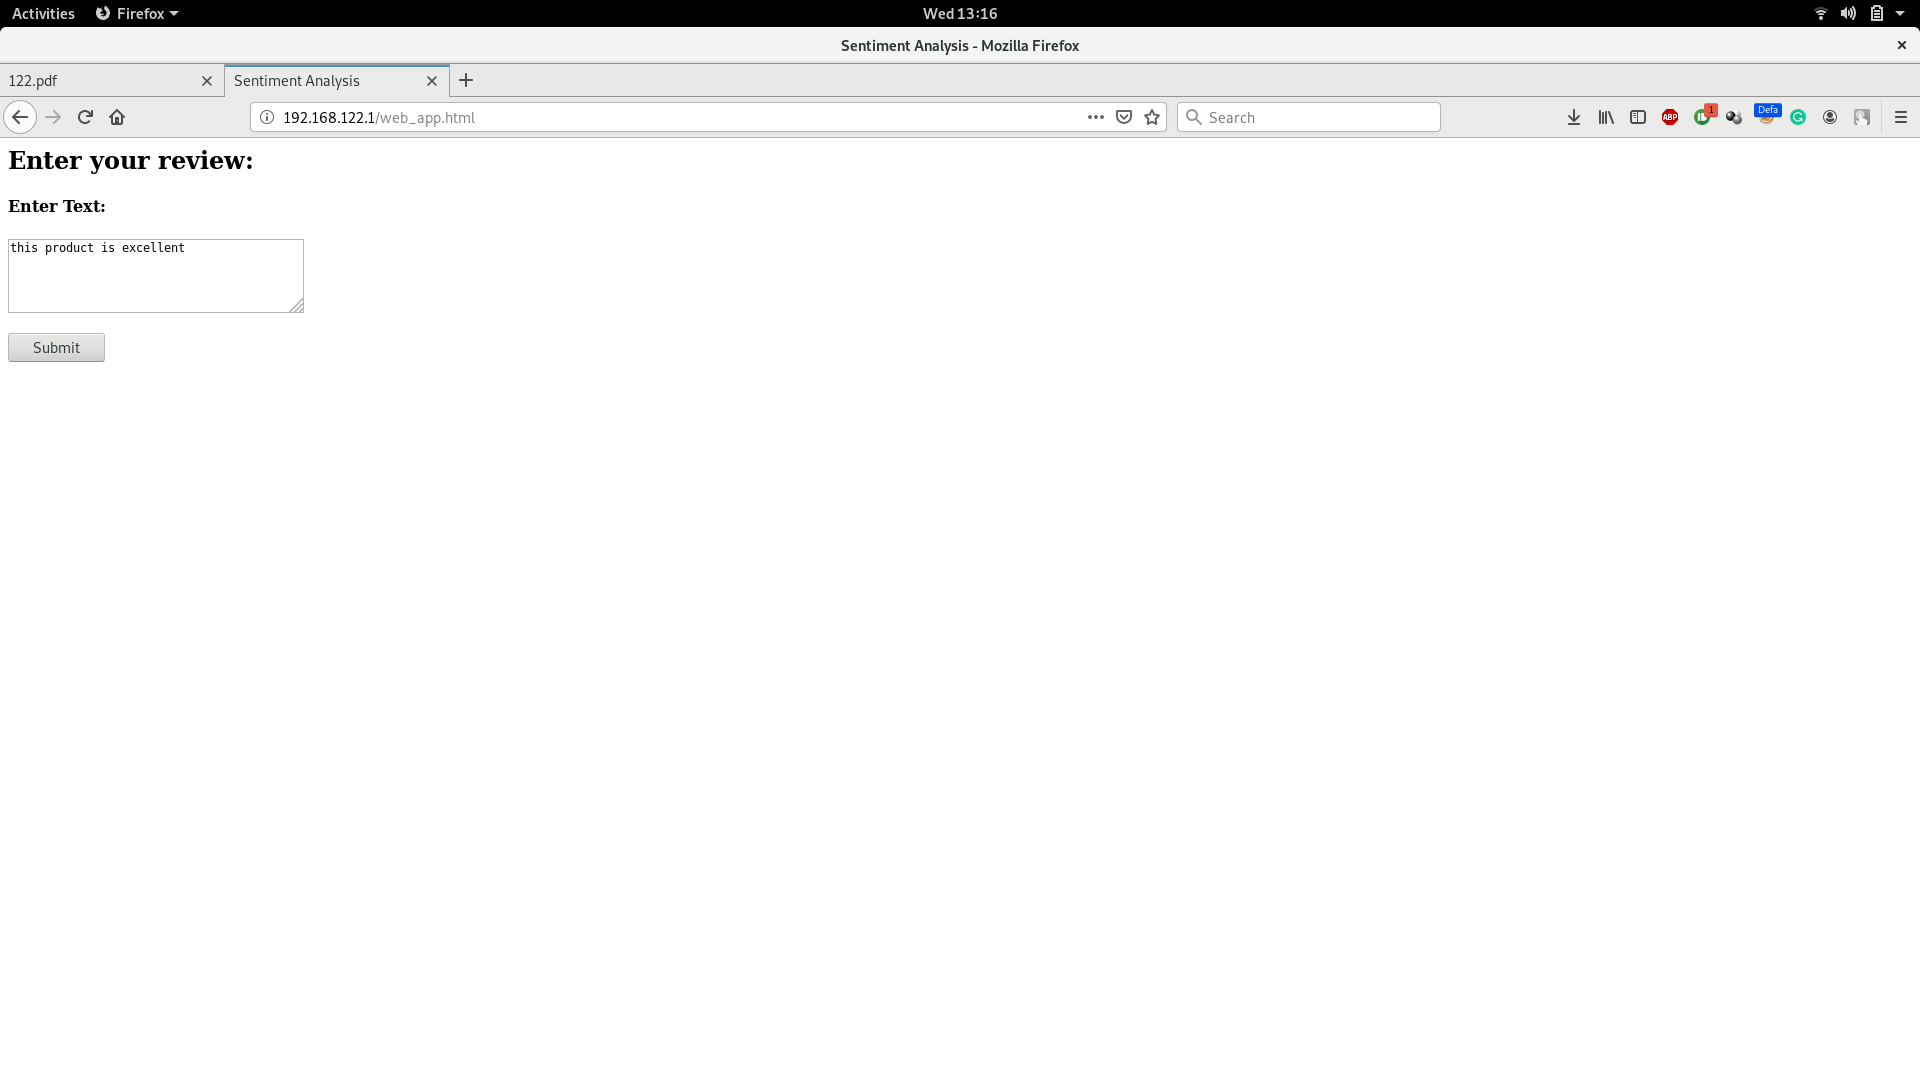
\includegraphics[height = 5cm,width=0.75\linewidth]{/root/Downloads/6}\\
	\caption{First review}
\end{figure}



\begin{figure}[h]
	\centering
	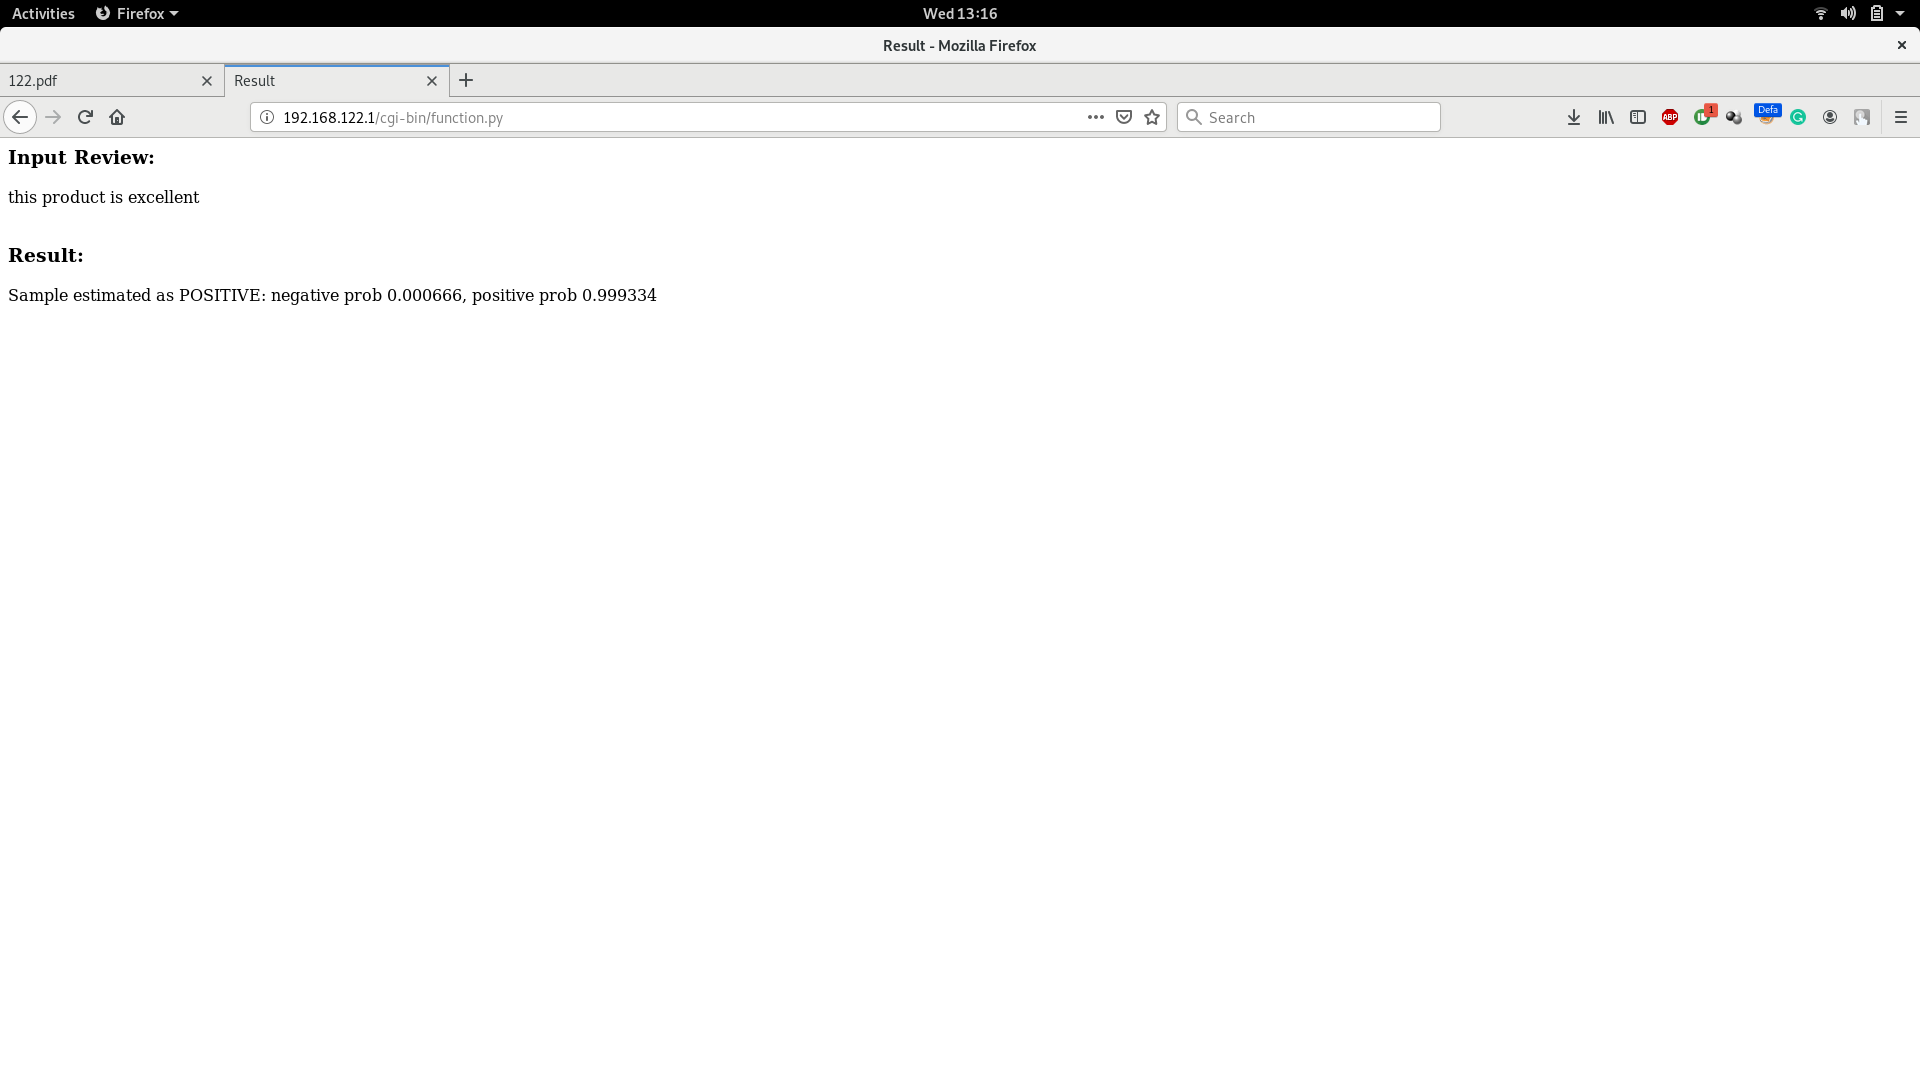
\includegraphics[height = 5cm,width=0.75\linewidth]{/root/Downloads/5}\\
	\caption{Result}
\end{figure}

\newpage


\begin{figure}[h]
	\centering
	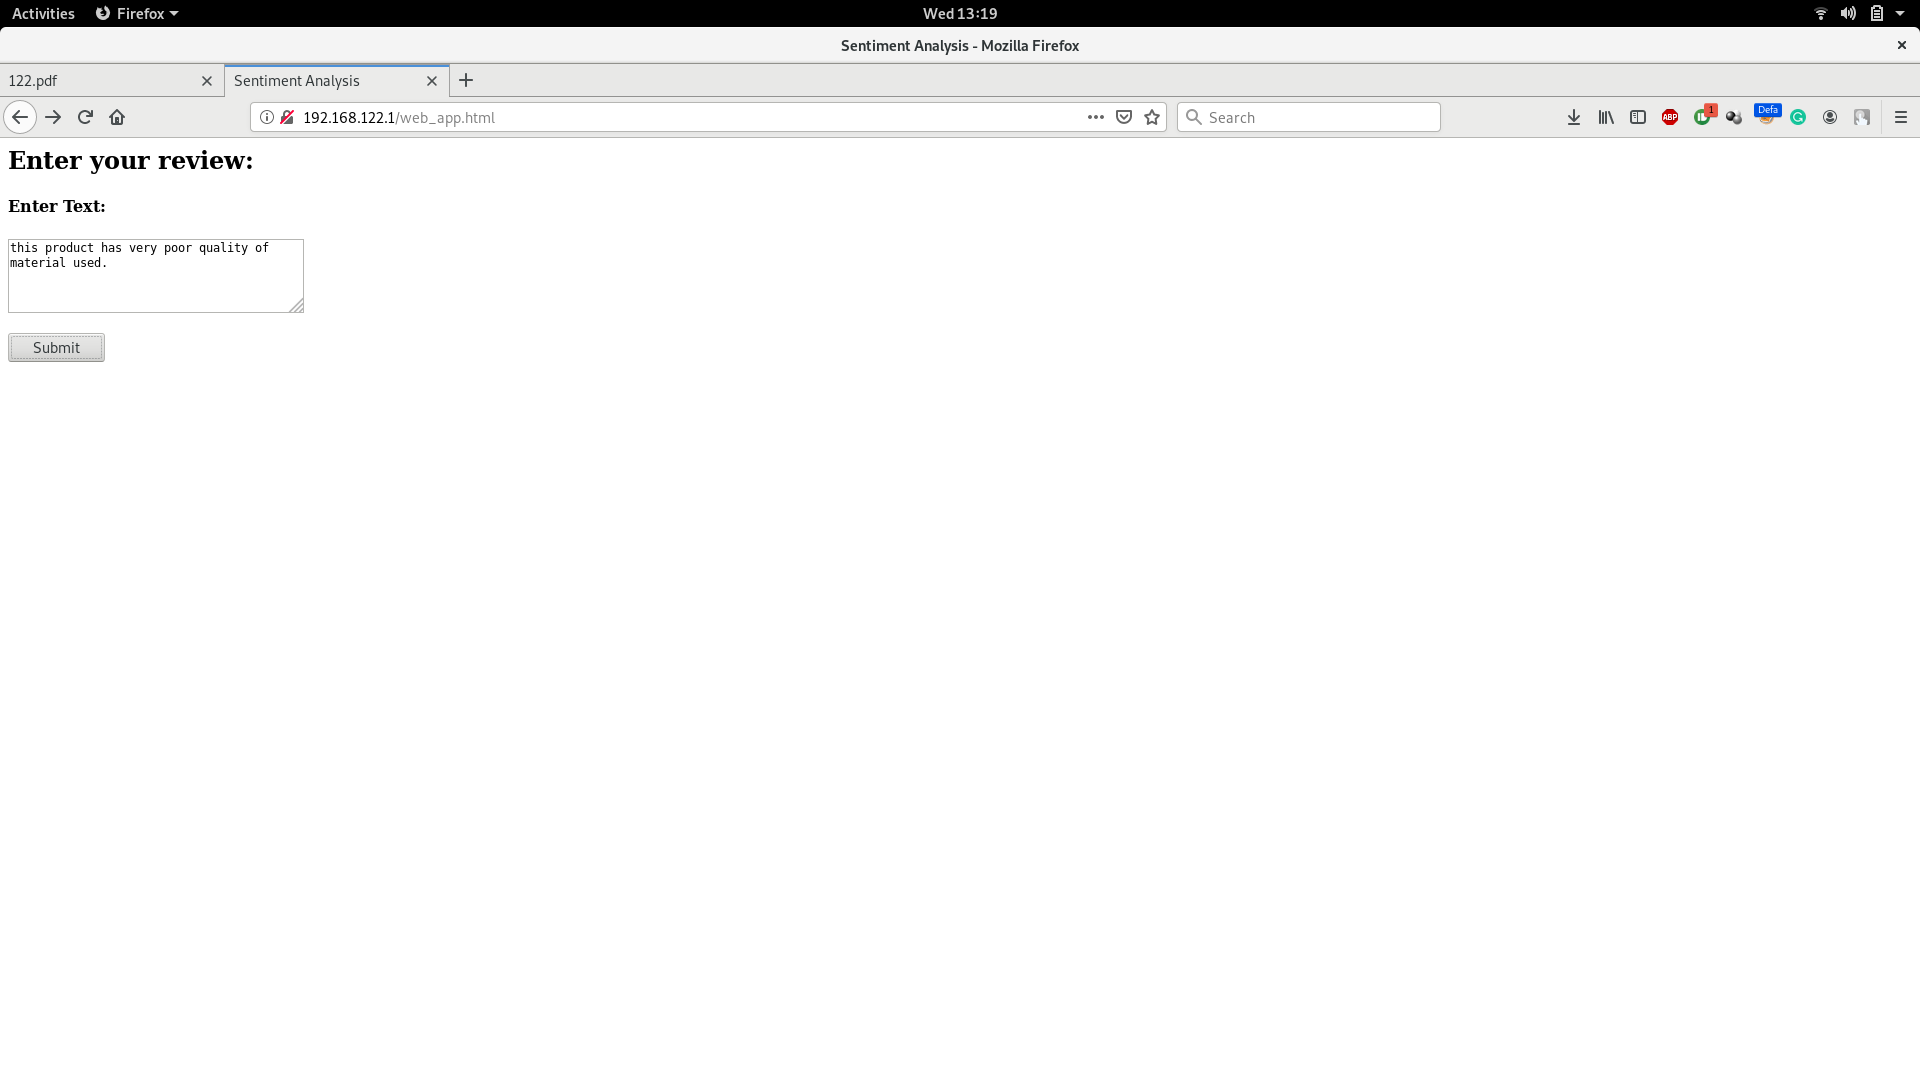
\includegraphics[height = 5cm,width=0.75\linewidth]{/root/Downloads/2}\\
	\caption{Second review}
\end{figure}



\begin{figure}[h]
	\centering
	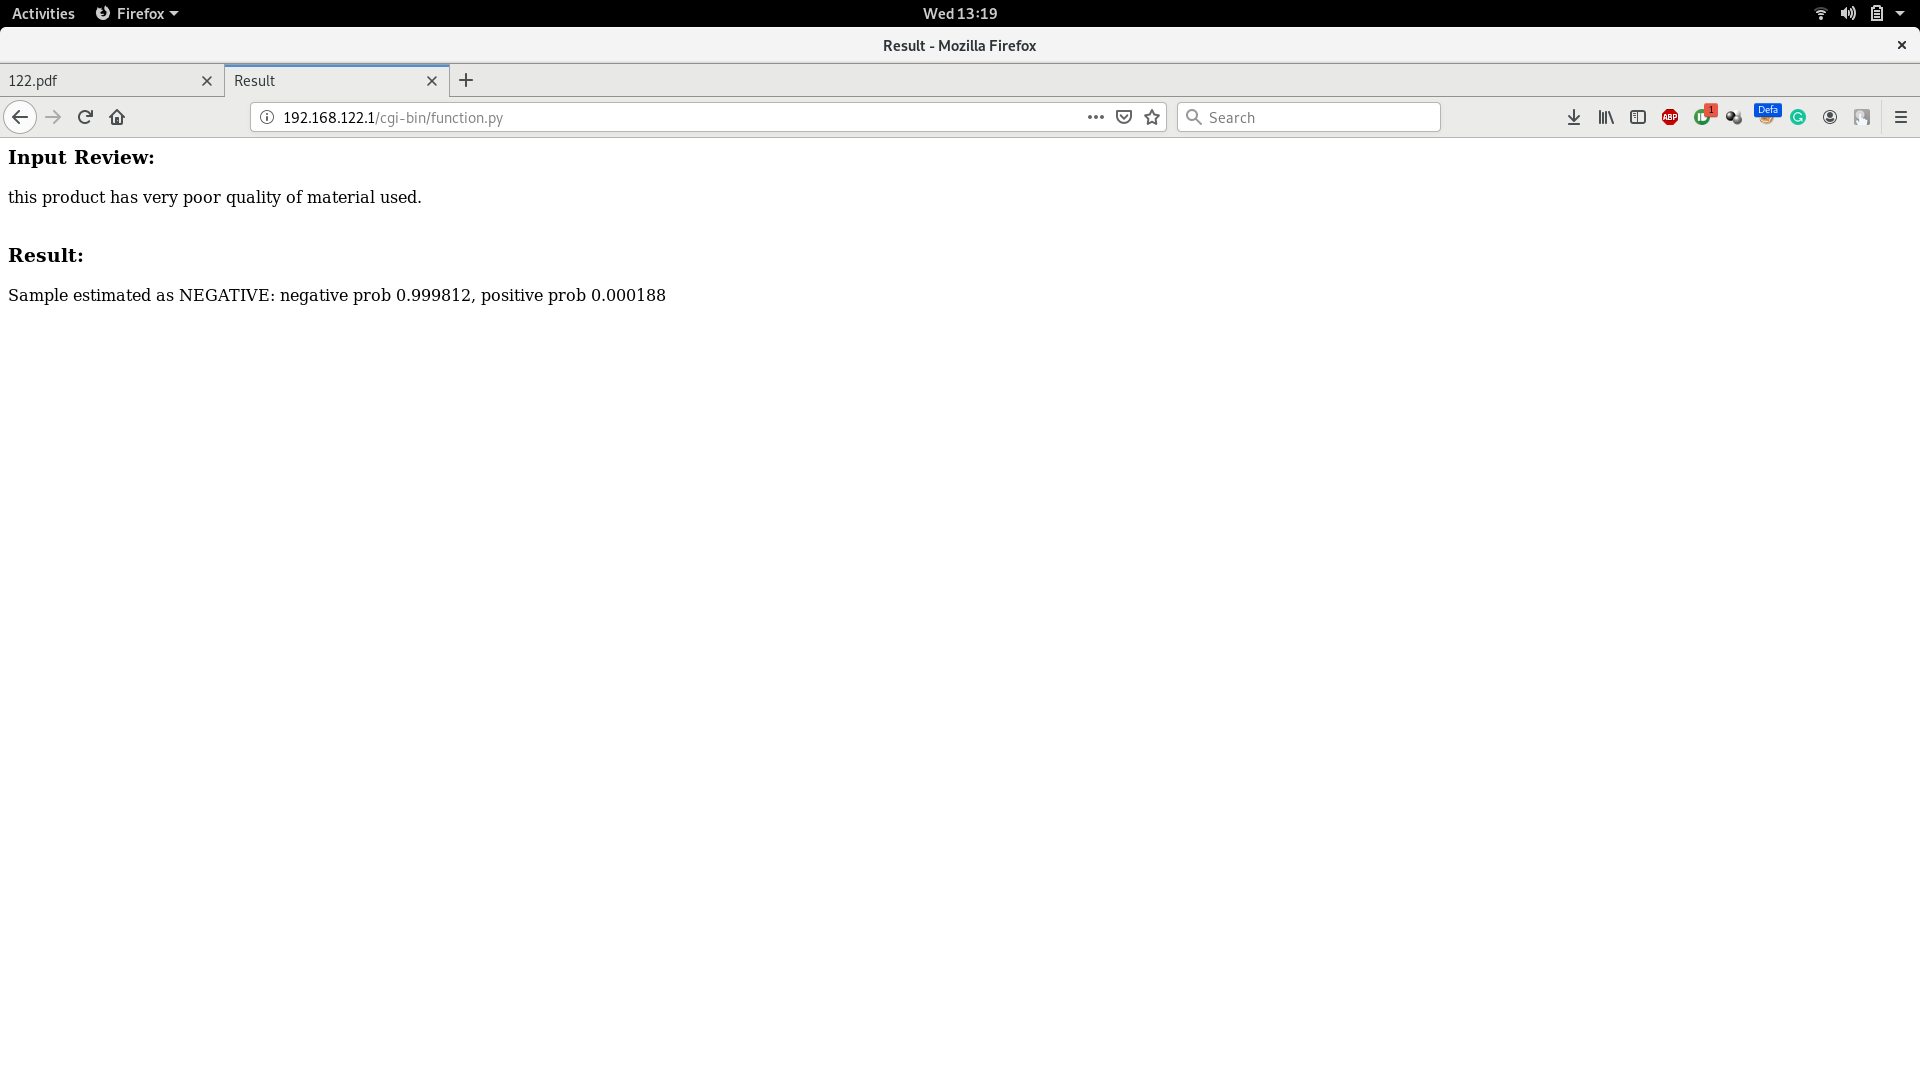
\includegraphics[height = 5cm,width=0.75\linewidth]{/root/Downloads/1}\\
	\caption{Result}
\end{figure}
In our web interface we don't have any character limit as we can insert as many characters we want.Our interface is successful in predicting the results.\\
In our interface when we use twisted reviews the result that we obtain are less accurate than those with less twisted reviews.


\newpage
\section{Conclusions and Future Work}
\justifying
Sentiment analysis deals with the classification of texts based on the sentiments they contain. This article focuses on a typical sentiment analysis model consisting of three core steps, namely data preparation, review analysis and sentiment classification, and describes representative techniques involved in those steps.Sentiment analysis is an emerging research area in text mining and computational linguistics, and has attracted considerable research attention in the past few years. Future research shall explore sophisticated methods for opinion and product feature extraction, as well as new classification models that can address the ordered labels property in rating inference. Applications that utilize results from sentiment analysis is also expected to emerge in the near future.\\

As we know in this competition era many companies in order to uphold the positions in the market are making False reviews on competitor's companies products. So in order to come over this situation we need to develop one strong false review detection system which will detect the false review made on the products and will ensure transparency among the users.

\bibliographystyle{unsrt}
\bibliography{new2}


\end{document}